\chapter{Anleitungen und Tests}\label{ch:Anleitungen}

\section{Anleitungen}

\glqq Elizitieren\grqq{}

\paragraph*{Glossar}

Glossar erstellen \url{https://www.lektorat-bachelorarbeit.de/glossar-erstellen/#:~:text=In%20einem%20Glossar%20sammelt%20man,die%20Erstellung%2C%20beantwortet%20dieser%20Text.} \\
It is possible to reference glossary entries as \gls{Immersion} as an example.

\paragraph{Bilder einfügen}
nach paragraph muss was stehen bevor das bild kommt

\begin{figure}[!h]
    \centering
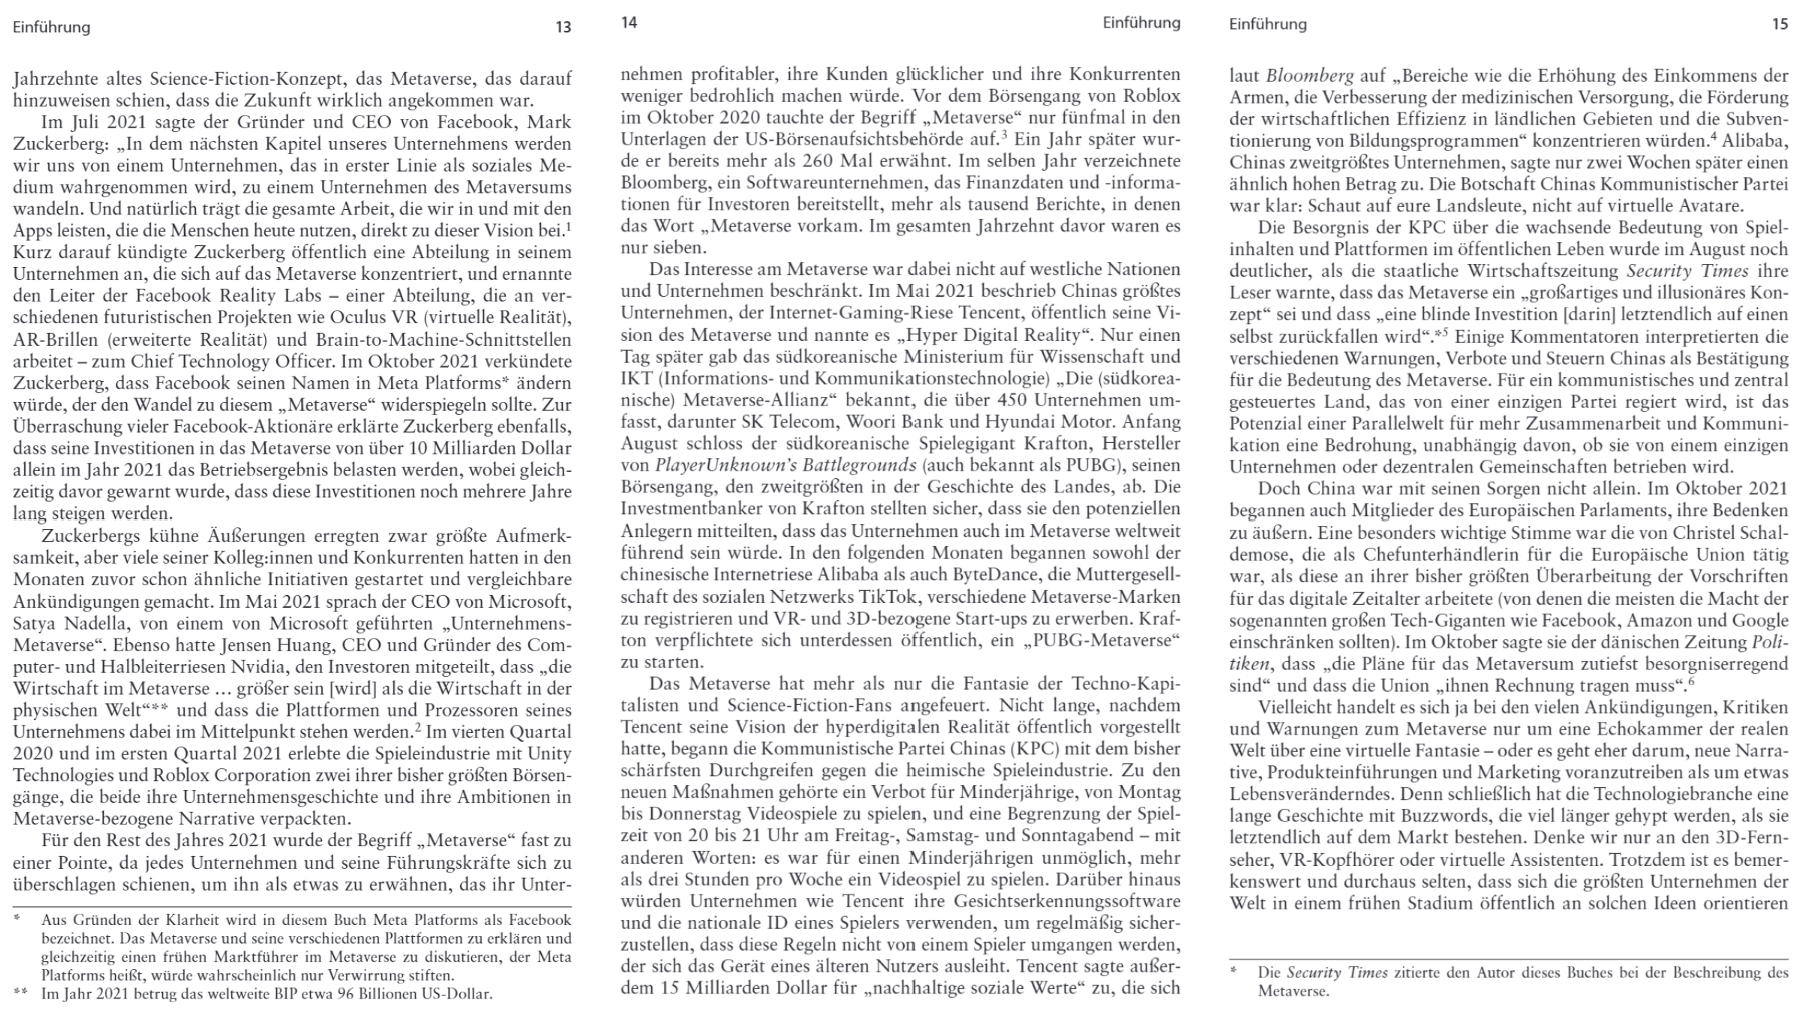
\includegraphics[width = 15cm]{figures/Das_Metaverse_uwearw13-15.png}
\caption{Das Metaverse und wie es alles revolutionieren wird}
\cite{Ball22}
\label{fig:testbild}
\end{figure}

%In this chapter, we're actually using some code!\\

%\begin{lstlisting}[language=Python,caption={This is an example of inline listing},captionpos=b]
%x = 1
%if x == 1:
%    # indented four spaces
%    print("x is 1.")

%\end{lstlisting}

%You can also include listings from a file directly:

%\lstinputlisting[language=Python,caption={This is an example of included listing},captionpos=b]{listings/example.py}


\section*{Tests}

Definitionen Metaverse \cite{Ball22}
\\Definitionen Metaverse \cite{Ball22a}
\\Definitionen Metaverse \cite{Drip22} \\
Seite 46 gegen wen Kämpfen wir \cite{Hypp22}\\
Psychologie hinter SocialEngeneering \cite{schu11}\\
\\

URL einfügen \url{https://ar5iv.labs.arxiv.org/html/2401.05569}


You can also write footnotes.\footnote{Footnotes will be positioned automatically.}

äüö
